\documentclass[12pt,a4paper]{article}
\usepackage[utf8]{inputenc}
%\usepackage[spanish]{babel}
\usepackage{amsmath}
\usepackage{amsfonts}
\usepackage{amssymb}
\usepackage{geometry}
\usepackage{tikz}
\usetikzlibrary{optics, angles, quotes, shapes.geometric, arrows.meta}
\geometry{left=2cm, right=2cm, top=2.5cm, bottom=2.5cm}

\begin{document}
	
	\begin{center}
		\textbf{METROLOGÍA ÓPTICA} \\
		\textbf{TAREA 5 y examen final.}
	\end{center}
	
	\vspace{0.5cm}
	\noindent
	\textbf{NOMBRE:}\rule{8cm}{0.4pt} \hfill \textbf{FECHA:}\rule{3cm}{0.4pt}
	
	\vspace{0.8cm}
	\noindent \textbf{INSTRUCCIONES.- Conteste de manera completa las siguientes preguntas.}
	
	\begin{enumerate}
		\item Explique los siguientes conceptos
		\begin{enumerate}
			\item \textbf{Holografía:} Es un método óptico que permite registrar y reconstruir tridimensionalmente la imagen de un objeto. Se basa en la interferencia de dos frentes de onda coherentes (un haz objeto y un haz de referencia) y en el fenómeno de difracción para recuperar la información topográfica.
			\item \textbf{Holograma:} Es el registro físico o la matriz digital donde queda codificado el patrón de interferencia microscópico. Este patrón almacena simultáneamente la intensidad (amplitud) y la fase del frente de onda electromagnético.
			\item \textbf{Holografía analógica y digital:} La holografía analógica utiliza emulsiones fotográficas fotosensibles para registrar el patrón, requiriendo iluminación con láser físico para su reconstrucción óptica. La holografía digital emplea un sensor optoelectrónico (CCD o CMOS) para adquirir el holograma y utiliza algoritmos matemáticos en una computadora para retro-propagar el campo óptico y reconstruir la imagen virtualmente.
			\item \textbf{Grabación y reconstrucción de un holograma:} La grabación (adquisición) es el proceso de capturar el patrón de intensidad resultante de la superposición coherente de la onda objeto y la de referencia. La reconstrucción consiste en multiplicar dicho holograma por un modelo numérico de la onda de referencia y propagarlo espacialmente (usando la integral de difracción) hacia el plano original para formar la imagen de amplitud y fase.
		\end{enumerate}
		
		\item Existen métodos numéricos para reconstruir un holograma, investigue cuales son y el principio de funcionamiento de ellos.\\
		\textbf{Aproximación de Fresnel:} Se basa en la integral de difracción de Fresnel-Kirchhoff evaluada en el régimen paraxial. Se implementa multiplicando matemáticamente el holograma por una fase esférica cuadrática (función chirp) y calculando una única Transformada Rápida de Fourier (FFT). En este método, el tamaño del píxel reconstruido depende directamente de la distancia de propagación $z$.\\
		\textbf{Método de Convolución:} Interpreta la propagación de Rayleigh-Sommerfeld como un filtro lineal invariante al desplazamiento. Calcula el campo difractado convolucionando el holograma con la respuesta al impulso del espacio libre en el dominio frecuencial. Suele usar dos o tres FFTs y su principal ventaja es que el tamaño del píxel reconstruido permanece constante independientemente de $z$.\\
		\textbf{Método del Espectro Angular (ASM):} Descompone el frente de onda capturado en un espectro de ondas planas mediante una FFT. Luego, aplica un núcleo exacto de propagación de fase a cada frecuencia espacial y regresa al dominio espacial con una FFT inversa. Es una solución rigurosa a la ecuación de Helmholtz, ideal para reconstrucciones a distancias muy cortas al no depender de aproximaciones paraxiales.
		
		\item Deduzca la ecuación para la transformada discreta de Fresnel.\\
		Partiendo de la integral analítica de propagación de Fresnel en el dominio continuo:
		\begin{align*} U'(x,y) =& \frac{i e^{-ikz}}{\lambda z} e^{\frac{-i\pi(x^2 + y^2)}{\lambda z}} \\ &\iint_{-\infty}^{\infty} A(\xi,\eta) e^{\frac{-i\pi(\xi^2 + \eta^2)}{\lambda z}} e^{i 2\pi\left( \frac{x\xi}{\lambda z} + \frac{y\eta}{\lambda z} \right)} d\xi d\eta \end{align*}
		Para discretizarla, consideramos un sensor digital con resolución de $N \times M$ píxeles y tamaños espaciales $\Delta\xi$ y $\Delta\eta$. Las coordenadas de la cámara se vuelven discretas: $\xi = n \Delta\xi$ y $\eta = m \Delta\eta$. Las coordenadas transversales del plano de reconstrucción escalan geométricamente conforme a la distancia $d$: $\Delta x' = \frac{\lambda d}{N \Delta\xi}$ y $\Delta y' = \frac{\lambda d}{M \Delta\eta}$. Evaluando las variables en las coordenadas discretas de matriz $(p, l)$, llegamos a la Transformada Discreta de Fresnel (SDFT):
		\begin{align*} U(p, l) =& \exp\left[ -i\pi \lambda d \left( \frac{p^2}{N^2 \Delta\xi^2} + \frac{l^2}{M^2 \Delta\eta^2} \right) \right] \\ &\times \sum_{n=0}^{N-1} \sum_{m=0}^{M-1} A(n, m) R^*(n, m) \exp\left[ -\frac{i\pi}{\lambda d} (n^2\Delta\xi^2 + m^2\Delta\eta^2) \right] \\ &\times \exp\left[ i 2\pi \left(\frac{p n}{N} + \frac{l m}{M}\right) \right] \end{align*}
		
		\item Explique el efecto Talbot y sus aplicaciones.\\
		El efecto Talbot (o fenómeno de autoimagen) es un efecto de difracción de campo cercano que se manifiesta cuando ondas planas incidentes de luz coherente atraviesan una estructura periódica, como una rejilla de difracción de Ronchi. A medida que el campo se propaga sin intervención de lentes, la interferencia origina réplicas exactas de la rejilla a distancias regulares a lo largo del eje óptico, conocidas como longitudes de Talbot. Se aplica activamente en la interferometría de Talbot para perfilar gradientes de índice de refracción, en la metrología para el escaneo tridimensional estructurado y en la caracterización de defectos en lentes e instrumentos ópticos.
		
		\item Deduzca las siguientes ecuaciones (longitud de Talbot) y explíquelas:
		\begin{enumerate}
			\item \[ z_T = \frac{2a^2}{\lambda} \]
			Esta ecuación define la distancia principal de Talbot bajo la aproximación paraxial. Si calculamos la diferencia de camino óptico (DCO) entre el haz difractado de orden cero y el de primer orden tras recorrer una distancia $z$. Para ángulos de difracción muy pequeños provocados por una rejilla de periodo $a$, se cumple que $\sin\theta \approx \theta = \frac{\lambda}{a}$. La diferencia de distancia geométrica recorrida es $\Delta L = \frac{z}{\cos\theta} - z$. Aproximando $\cos\theta \approx 1 - \frac{\theta^2}{2}$, tenemos que $\Delta L \approx z(1 + \frac{\theta^2}{2}) - z = \frac{z\theta^2}{2}$. Para que los haces interfieran de forma idéntica a la salida de la rejilla (generando la autoimagen), la diferencia de camino debe ser igual a una longitud de onda ($\Delta L = \lambda$). Igualando y sustituyendo $\theta$: $z \frac{\lambda^2}{2a^2} = \lambda \implies z_T = \frac{2a^2}{\lambda}$.
			
			\item \[ z = \frac{a}{\pm \sqrt{1 - \frac{\lambda^2}{a^2}}} \]
			Esta expresión se deduce analizando la relación geométrica transversal de propagación libre del haz difractado sin aplicar restricciones paraxiales. Sabemos que un haz se dispersa con un ángulo de difracción tal que $\sin\theta = \frac{\lambda}{a}$. Por identidad trigonométrica, el coseno del ángulo exacto es $\cos\theta = \pm\sqrt{1 - (\frac{\lambda}{a})^2}$. Si queremos calcular a qué distancia $z$ el haz se desplaza transversalmente una distancia igual a un periodo espacial $a$ respecto al eje óptico, aplicamos la geometría del triángulo rectángulo: $\tan\theta = \frac{\text{Cateto Opuesto}}{\text{Cateto Adyacente}} = \frac{a}{z}$. Despejando $z = \frac{a}{\tan\theta} = a \frac{\cos\theta}{\sin\theta}$. Al sustituir las funciones angulares obtenemos la proyección del vector de onda que se utiliza para calcular las correcciones de propagación en la teoría exacta de Rayleigh.
		\end{enumerate}
		
		\item Describa completamente los siguientes temas:
		\begin{enumerate}
			\item \textbf{Luz Estructurada:} Tecnología de visión por computadora y metrología óptica que consiste en proyectar de manera activa patrones codificados de luz sobre la superficie de una escena. Analizando computacionalmente cómo se distorsionan estos patrones sobre los volúmenes del objeto, el sistema recupera coordenadas espaciales 3D exactas de forma no invasiva.
			\item \textbf{Técnicas y aplicaciones de luz estructurada:} Las metodologías primarias incluyen codificaciones binarias, codificaciones N-ary, triangulación por Moiré y Perfilometría de Proyección de Franjas (FPP). Estas técnicas se aplican ampliamente en la inspección de control de calidad industrial, ingeniería inversa, modelado de prótesis biomédicas y la medición precisa de rugosidades superficiales.
			\item \textbf{Técnica de proyección de franjas:} Consiste en utilizar proyectores de tecnología DLP o LCD para iluminar el objeto con franjas de perfil de intensidad cosenoidal. La cámara captura imágenes con la deformación generada por la topografía. Mediante algoritmos de demodulación de corrimiento de fase (Phase Shifting Profilometry), se calcula una fase óptica analítica que se mapea directamente a las variaciones milimétricas de la altura.
			\item \textbf{Técnica de moiré, incluyendo sus aplicaciones:} Aprovecha el fenómeno de interferencia visual originado por la superposición multiplicativa de dos estructuras periódicas finas, generando un patrón secundario "fluctuante" de baja frecuencia. En sistemas de "Moiré por sombra", una rejilla se sitúa muy cerca del objeto, y la sombra de dicha rejilla interfiere con la rejilla física originando contornos de nivel de elevación. Sus principales aplicaciones son el análisis de deformación en materiales (medición de tensiones en el plano) y la topografía biomédica de cuerpos completos como en los exámenes de escoliosis espinal.
		\end{enumerate}
		
		\item Deduzca la siguiente ecuación y explique cada término.
		\[ h(x,y) = \frac{\phi(x,y)}{2\pi} \frac{p}{\tan \alpha} \]
		\textbf{Deducción y explicación:} Al realizar el mapeo de fase a altura en un montaje de proyección de franjas cruzadas, la altura superficial del objeto $h(x,y)$ induce un desplazamiento espacial o lateral $u(x)$ del patrón de luz respecto a un plano de referencia calibrado. Por simple trigonometría del ángulo de triangulación del proyector $\alpha$, tenemos que $u(x) = h(x,y) \tan \alpha$. Al proyectar franjas sinusoidales espaciales, sabemos que un desplazamiento lateral equivalente a un periodo completo $p$ se manifiesta en la fase óptica como un ciclo completo de $2\pi$ radianes. Así, el cambio de fase medido es directamente proporcional: $\phi(x,y) = \frac{2\pi}{p} u(x)$. Al sustituir la equivalencia de $u(x)$ en la ecuación angular se obtiene $\phi(x,y) = \frac{2\pi}{p} h(x,y) \tan \alpha$. Despejando matemáticamente $h(x,y)$, se demuestra la ecuación.\\
		\textbf{Términos:} $h(x,y)$ corresponde a la altura en el mapa topográfico 3D reconstruido, $\phi(x,y)$ es la fase óptica continua calculada mediante algoritmos, $p$ es el periodo espacial calibrado del patrón sobre el plano, y $\alpha$ es el ángulo oblicuo entre el proyector y el eje de visión de la cámara.
		
		\item Explique los siguientes términos: fase de envoltura, fase desenrollada, patrones de franjas, periodo del patrón de franjas.
		\begin{itemize}
			\item \textbf{Fase de envoltura (Wrapped phase):} Es el resultado crudo de aplicar un cálculo de arco-tangente en la evaluación del holograma o patrón (ej. $\arctan2$). Limita matemáticamente todos los ángulos al intervalo principal de $[-\pi, \pi)$, por lo que la representación gráfica sufre "saltos" discontinuos en forma de dientes de sierra.
			\item \textbf{Fase desenrollada (Unwrapped phase):} Representa la fase física espacialmente continua del objeto. Se obtiene sumando o restando algorítmicamente múltiplos enteros correctivos de $2\pi$ a la fase de envoltura para suprimir sus saltos artificiales, y es el factor clave proporcional a la altura topográfica.
			\item \textbf{Patrones de franjas:} Son rejillas ópticas periódicas estructuradas empleadas como sonda metrológica. Son bandas alternadas que modulan la intensidad desde regiones oscuras hasta regiones de brillo máximo en un régimen cuadrado, triangular o sinusoidal armónico.
			\item \textbf{Periodo del patrón de franjas:} Dimensión lineal física evaluada ortogonalmente que define la longitud de un ciclo completo de repetición del patrón; es decir, la métrica espacial entre el pico central de una franja de máxima brillantez y el pico de su franja contigua inmediata.
		\end{itemize}
		
		\item Describa el método: Holografía sin lentes.\\
		Es un esquema de microscopía digital avanzada que omite enteramente el uso de lentes ópticas objetivas entre la muestra y el sensor para evitar cualquier límite numérico de apertura y aberraciones esféricas. Consiste en emplear una fuente puntual sumamente divergente (como la luz emergente del núcleo de una fibra óptica monomodo). El haz ilumina una muestra translúcida; la parte de la luz que dispersa la muestra actúa como onda objeto, mientras que la que transita inalterada cumple la función de la onda de referencia. Ambas interfieren co-linealmente de manera directa sobre un sensor CCD/CMOS adyacente. La imagen 3D final se recupera propagando este patrón mediante un "autoenfoque" algorítmico que calcula la Transformada Discreta de Fresnel en la computadora.
		
		\item Deduzca las siguientes ecuaciones para el efecto moiré.\\
		En un entorno óptico configurado para Moiré por sombra, se debe cuantificar la topografía $h(x,y)$. Considerando un haz colimado que incide con un ángulo $\alpha$ y una cámara que observa el plano en un ángulo $\beta$ (ambos respecto a la normal del arreglo). Un punto físico proyectado en el fondo se moverá una distancia trasversal o desviación $u(x)$ que es la suma del vector incidido al objeto y el vector reflejado hasta la rejilla. Analizando los triángulos de profundidad, $u(x) = h(x,y) \tan \alpha + h(x,y) \tan \beta = h(\tan\alpha + \tan\beta)$. 
		El efecto moiré genera la franja topográfica de contorno o el máximo de orden $N$ cada vez que el desplazamiento lateral equivale de manera precisa a un múltiplo del periodo espacial $p$ de la rejilla, es decir: $u(x) = N p$. 
		Igualando el modelo de orden de franja con la descripción geométrica obtenemos: $h(x,y)(\tan\alpha + \tan\beta) = N p$. Al despejar, deducimos el relieve de manera inequívoca:
		\[ h(x,y) = \frac{Np}{\tan \alpha + \tan \beta} \]
		
		\item Describa completamente los siguientes métodos para recuperar la forma:
		\begin{enumerate}
			\item \textbf{Dos puntos de iluminación:} Es una técnica interferométrica dual donde la medición de topografía se efectúa mediante la conmutación de dos haces incidentes a ángulos precisos (iluminación iterativa). Al adquirir los perfiles de interferencia de ambos estados con respecto a la visual de la cámara y sustraerlos, se cancelan las aberraciones ambientales comunes y el resultado directo de la diferencia de fase ($\Delta \phi$) se vuelve proporcional enteramente al relieve de profundidad del espécimen, estableciendo mapas de alta sensibilidad para relieves rugosos.
			\item \textbf{Dos longitudes de onda:} Para saltar la limitante de ambigüedad metrológica inducida por topografías abruptas que desbordan un ciclo de fase de un láser estándar de prueba, este método irradia coherentemente el volumen con dos longitudes de onda próximas, $\lambda_1$ y $\lambda_2$. Por el fenómeno de batimiento, se genera un mapa de ruido equivalente que reacciona dictado por una longitud de onda sintética muy superior dada por $\Lambda = \frac{\lambda_1 \lambda_2}{|\lambda_1 - \lambda_2|}$. Esta técnica recupera la estructura macroscópica uniendo la resolución sin saltos de $\Lambda$ con el fino grado de los escalones elementales individuales.
		\end{enumerate}
		
		\item Realice los arreglos ópticos para : 
		\begin{enumerate}
			\item \textbf{Holografía sin lentes}
			\vspace{0.3cm}
			\begin{center}
				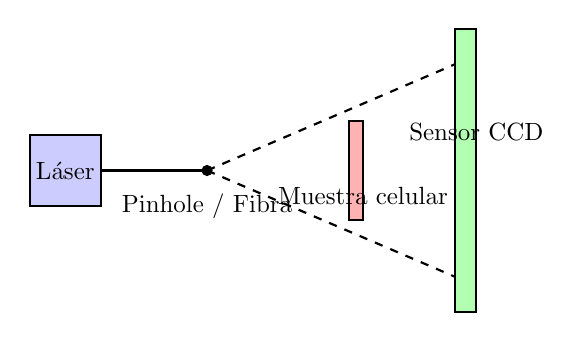
\begin{tikzpicture}[scale=0.9, transform shape]
					\draw[thick, fill=blue!20] (0,0) rectangle (1,1) node[midway] {Láser};
					\draw[thick] (1,0.5) -- (2.5,0.5);
					\filldraw[black] (2.5, 0.5) circle (2pt) node[below=0.2cm] {Pinhole / Fibra};
					\draw[thick, dashed] (2.5, 0.5) -- (6, 2);
					\draw[thick, dashed] (2.5, 0.5) -- (6, -1);
					\draw[thick, fill=red!30] (4.5, -0.2) rectangle (4.7, 1.2) node[below=0.8cm] {Muestra celular};
					\draw[thick, fill=green!30] (6, -1.5) rectangle (6.3, 2.5) node[below=1.2cm] {Sensor CCD};
				\end{tikzpicture}
			\end{center}
			\vspace{0.5cm}
			
			\item \textbf{Holografía digital interferométrica (Mach-Zehnder)}
			\vspace{0.3cm}
			\begin{center}
				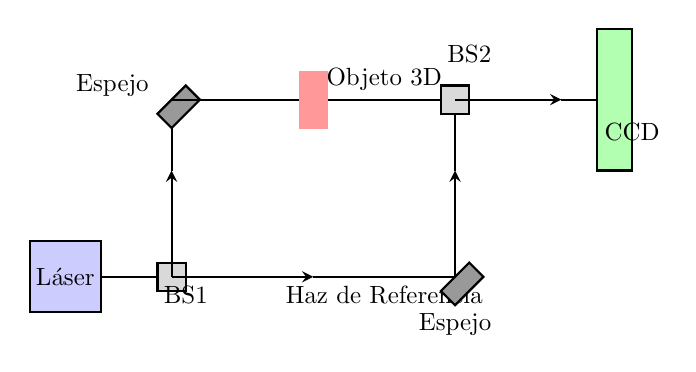
\begin{tikzpicture}[scale=0.9, transform shape]
					\draw[thick, fill=blue!20] (-2,-1) rectangle (-1,0) node[midway] {Láser};
					\draw[thick] (-1,-0.5) -- (0,-0.5);
					\draw[thick, fill=gray!30] (-0.2,-0.7) rectangle (0.2,-0.3) node[below=0.2cm] {BS1};
					\draw[thick, ->, >=stealth] (0,-0.5) -- (2,-0.5);
					\draw[thick] (2,-0.5) -- (4,-0.5) node[midway, below] {Haz de Referencia};
					\draw[thick, ->, >=stealth] (0,-0.5) -- (0,1);
					\draw[thick] (0,1) -- (0,2);
					\draw[thick, fill=gray!80] (-0.2,1.8) -- (0.2,2.2) -- (0.4,2.0) -- (0,1.6) -- cycle;
					\node[left] at (-0.2,2.2) {Espejo};
					\draw[thick, ->, >=stealth] (0,2) -- (2,2);
					\draw[thick] (2,2) -- (4,2) node[midway, above] {Objeto 3D};
					\filldraw[red!40] (1.8,1.6) rectangle (2.2,2.4);
					\draw[thick, fill=gray!80] (3.8,-0.7) -- (4.2,-0.3) -- (4.4,-0.5) -- (4,-0.9) -- cycle;
					\node[below] at (4,-0.9) {Espejo};
					\draw[thick, ->, >=stealth] (4,-0.5) -- (4,1);
					\draw[thick] (4,1) -- (4,2);
					\draw[thick, fill=gray!30] (3.8,1.8) rectangle (4.2,2.2) node[above=0.2cm] {BS2};
					\draw[thick, ->, >=stealth] (4,2) -- (5.5,2);
					\draw[thick] (5.5,2) -- (6,2);
					\draw[thick, fill=green!30] (6,1) rectangle (6.5,3) node[below=1.2cm] {CCD};
				\end{tikzpicture}
			\end{center}
			\vspace{0.5cm}
			
			\item \textbf{Proyección de Franjas}
			\vspace{0.3cm}
			\begin{center}
				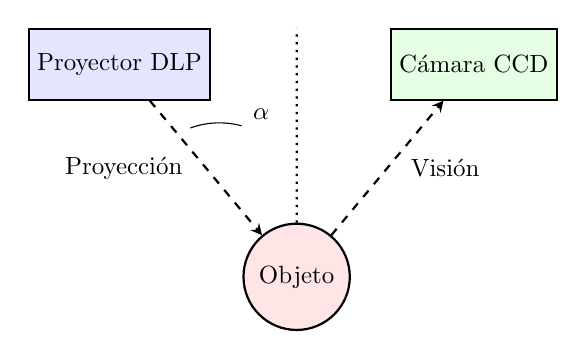
\begin{tikzpicture}[scale=0.9, transform shape]
					\node[draw, thick, fill=blue!10, minimum height=1cm] (proj) at (0,3) {Proyector DLP};
					\node[draw, thick, fill=green!10, minimum height=1cm] (cam) at (5,3) {Cámara CCD};
					\node[draw, thick, circle, fill=red!10, minimum size=1.5cm] (obj) at (2.5,0) {Objeto};
					\draw[->, >=stealth, thick, dashed] (proj) -- (obj) node[midway, left=0.2cm] {Proyección};
					\draw[->, >=stealth, thick, dashed] (obj) -- (cam) node[midway, right=0.2cm] {Visión};
					\draw[dotted, thick] (obj) -- (2.5,3.5);
					\draw (1,2.1) arc (110:75:1.2);
					\node at (2, 2.3) {$\alpha$};
				\end{tikzpicture}
			\end{center}
			\vspace{0.5cm}
			
			\item \textbf{Moiré por sombras}
			\vspace{0.3cm}
			\begin{center}
				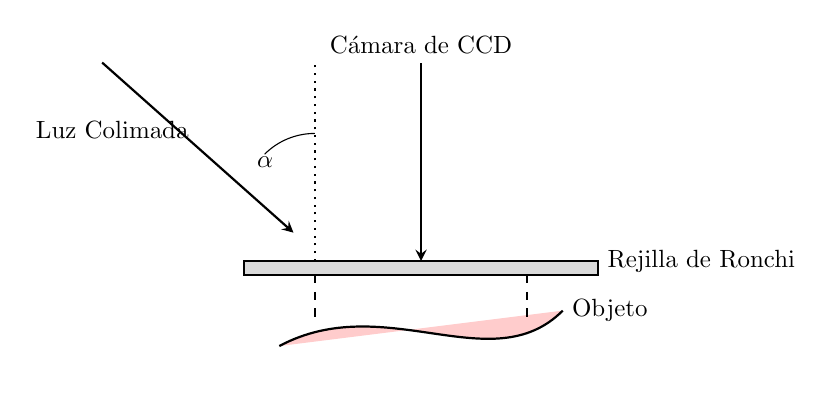
\begin{tikzpicture}[scale=0.9, transform shape]
					\draw[thick, ->, >=stealth] (-1.5,3) -- (1.2,0.6) node[midway, above left] {Luz Colimada};
					\draw[thick, fill=gray!30] (0.5,0) rectangle (5.5,0.2) node[right] {Rejilla de Ronchi};
					\draw[thick, fill=red!20] (1,-1) .. controls (2.5,-0.2) and (4,-1.5) .. (5,-0.5) node[right] {Objeto};
					\draw[thick, dashed] (1.5, 0) -- (1.5, -0.6);
					\draw[thick, dashed] (4.5, 0) -- (4.5, -0.7);
					\draw[thick, <-, >=stealth] (3,0.2) -- (3,3) node[above] {Cámara de CCD};
					\draw[dotted, thick] (1.5,0.2) -- (1.5,3);
					\draw (1.5,2) arc (90:135:1);
					\node at (0.8, 1.6) {$\alpha$};
				\end{tikzpicture}
			\end{center}
		\end{enumerate}
	\end{enumerate}
	
\end{document}
